\documentclass[a4paper,english,12pt]{article}   	% use }amsart} instead of }article} for AMSLaTeX format
 \usepackage{%
	amsmath,%
	amsfonts,%
	amssymb,%
	amsthm,%
	hyperref,%
	url,%
	latexsym,%
	epsfig,%
	graphicx,%
	psfrag,%
	subfigure,%	
	color,%
	tikz,%
	pgf,%
	pgfplots,%
	pgfplotstable,%
	pgfpages,%
	proofs%
}

\usepgflibrary{shapes}
\usetikzlibrary{%
  arrows,%
	backgrounds,%
	chains,%
	decorations.pathmorphing,% /pgf/decoration/random steps | erste Graphik
	decorations.text,%
	matrix,%
  positioning,% wg. " of "
  fit,%
	patterns,%
  petri,%
	plotmarks,%
  scopes,%
	shadows,%
  shapes.misc,% wg. rounded rectangle
  shapes.arrows,%
	shapes.callouts,%
  shapes%
}

\theoremstyle{plain}
\newtheorem{thm}{Theorem}[section]
\newtheorem{lem}[thm]{Lemma}
\newtheorem{prop}[thm]{Proposition}
\newtheorem{cor}[thm]{Corollary}

\theoremstyle{definition}
\newtheorem{defn}[thm]{Definition}
\newtheorem{conj}[thm]{Conjecture}
\newtheorem{exmp}[thm]{Example}
\newtheorem{assum}[thm]{Assumptions}

%\theoremstyle{remark}
\newtheorem{rem}{Remark}
\newtheorem{note}{Note}

\makeatletter
\def\th@plain{%
  \thm@notefont{}% same as heading font
  \itshape % body font
}
\def\th@definition{%
  \thm@notefont{}% same as heading font
  \normalfont % body font
}
\makeatother
\date{}
\geometry{letterpaper}                   		% ... or a4paper or a5paper or ...


\title{Lecture 12 : Topological Spaces}
\author{}

\begin{document}
\maketitle
%\section{}
%\subsection{}
\section{Topological Spaces}
Topology generalizes notion of distance and closeness etc. 
\begin{defn} A \textbf{topology} on a set $X$ is a collection $\T$ of subsets of $X$ having the following properties.
\begin{enumerate}
\item $\emptyset$ and $X$ are in $\T$.
\item The union of the elements of any sub-collection of $\T$ is in $\T$.
\item The intersection of elements of any finite sub-collection of $\T$ is in $\T$. 
\end{enumerate}
A set $X$ for which a topology $\T$ has been specified is called a \textbf{topological space}, denoted $(X,\T)$.
\end{defn}

\begin{defn} If $X$ is a topological space with topology $\T$, we say that a subset $U$ of $X$ is an \textbf{open set} of $X$ if $U$ belongs to the collection $\T$.
\end{defn}

\begin{figure}[hhhh]
 \centering
 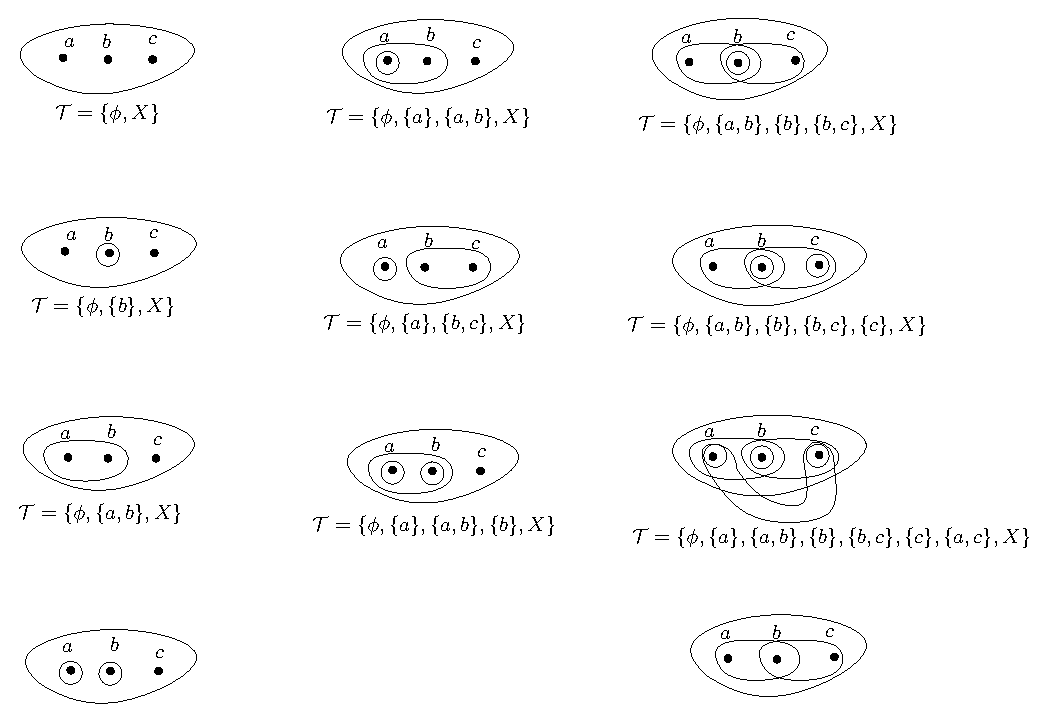
\includegraphics[width=\textwidth]{fig133.eps}
	\caption{Different collections of subsets of $X = \{a,b,c\}$. Last two subsets are not topologies.}
	\label{Fig:ExampleTopologies}
\end{figure}

\begin{exmp} Let $X$ be any set. 
\begin{enumerate}
	\item Let $X = \{a,b,c\}$. Different collections of subsets of $X$ are shown in the Figure~\ref{Fig:ExampleTopologies}. First nine of these collections are topologies and last two are not.
	\item Power set $\mathcal{P}(X)$ is a topology called the \textbf{discrete topology}.
	\item Collection $\T =\{\emptyset,X\}$ is a topology called the \textbf{indiscrete topology} or the \textbf{trivial topology}.
	\item  We define \textbf{finite complement topology} on $X$ as
	\begin{align*}
	\T_f = \{U \subseteq X : X{\setminus}U \text{ is finite or } X{\setminus}U = X\}. 
	\end{align*}
	We will show $\T_f$ is a topology.
	\begin{description}
		\item[Membership of $\emptyset$ and $X$.] Since $X{\setminus}\emptyset = X$, we have $\emptyset \in \T_f$. Similarly, $X \in \T_f$ since $X{\setminus}X = \emptyset$ is finite. 
		\item[Closure under arbitrary union.] 	Let $\{U_i: i \in I \}$ be an indexed family of elements in $\T_f$, with their union $\cup_{j \in I}U_j$ denoted by $U$. If $U_i = \emptyset$ for all $i \in I$, then there is nothing to show. Else, there exists $i \in I$ such that $X{\setminus}U_i$ is finite.  %To show that the union of any sub-collection $I$ of $U_i$ is in $\T_f$ 
Notice that
\begin{align*}
X{\setminus}U = X\setminus\bigcup_{j \in I}U_j=\bigcap_{j \in {I}}(X\setminus U_j) \subseteq (X\setminus U_i).
\end{align*}
Since $X\setminus U_i$ is finite, so is $X{\setminus}U$. It follows that union $U \in \T_f$. 
	\item[Closure under finite intersection.] For a finite index set $F$, consider $\{U_i: i \in F\}$ non-empty elements of $\T_f$, with their intersection $\cap_{i=1}^{n}U_i$ denoted by $V$. We notice that
\begin{align*} 
X{\setminus}V = X{\setminus}\bigcap_{i = 1}^nU_i=\bigcup_{i = 1}^n(X{\setminus}U_i).
\end{align*}
Since finite union of finite sets is finite, $V \in \T_f$. 
	\end{description}
	\item  We define \textbf{co-countable topology} on $X$ as
	\begin{align*}
	\T_c=\{U \subseteq X: X{\setminus}U \text{ countable or } X{\setminus}U =X \}.
	\end{align*} 
\end{enumerate} 
\end{exmp}

\begin{defn}  Let $\T, \T'$ be topologies on a set $X$. We say that topology $\T'$ is 
\begin{enumerate}
	\item \textbf{finer} than $\T$, if $\T \subseteq \T'$,
	\item \textbf{strictly finer} than $\T$, if  $\T \subset \T'$,
	\item is \textbf{comparable} to $\T$, if either $\T' \subseteq \T$ or $\T \subseteq \T'$.
\end{enumerate}
We say $\T$ is \textbf{coarser} or \textbf{strictly coarser} in above two cases, respectively. 
\end{defn}
\begin{defn}
 If $\T \subseteq \T'$, then we say that $\T'$ is \textbf{larger} than $\T$, and $\T$ is \textbf{smaller} than $\T$.
\end{defn}
\begin{rem} Topologies are not always comparable. In Figure~\ref{Fig:ExampleTopologies}, topology in first row and first column is coarser than all topologies, and topology in third row and third column is finer than all topologies. Topology in the second row and second column is not comparable, to other two topologies in the third row.
\end{rem}

\section{Basis for a Topology}
Specifying whole collection of open sets is prohibitive at times. One can specify a smaller collection of subsets of $X$ and define topology using them.
\begin{defn}
 If $X$ is a set, a \textbf{basis} for a topology on $X$ is a collection $\B$ of subsets of $X$, called \textbf{basis elements}, such that 
 \begin{enumerate}
  \item for all $x \in X$, there exists $B \in \B$ such that $x \in \B$,
  \item for $B_1, B_2 \in \B$ and $x \in B_1 \cap B_2$, there exists $B_3 \in \B$ such that $x \in B_3 \subseteq B_1 \cap B_2$.
 \end{enumerate}
	If $\B$ satisfies these two conditions, we define the topology \textbf{$\T$ generated by $\B$} as follows. A subset $U$ of $X$ is called open in $X$, if for each $x \in U$, there exists $B \in \B$ such that $x \in B \subseteq U$. 
\end{defn}
\begin{rem} Observe that $\B \subseteq \T$.
\end{rem}
 
\begin{lem} Collection $\T$ generated by basis $\B$ is a topology on $X$. 
\end{lem}
\begin{proof} Let $\T$ be the collection of subsets of $X$ generated by the basis $\B$ on $X$. 
	\begin{description}
		\item[Membership of $\emptyset$ and $X$.] Let $U$ be an empty set, in this case $U$ vacuously belongs to $\T$. On the other hand, for all $x \in X$, there exists $B$ such that $x \in B \subseteq X$ by definition of basis $\B$. 
		\item[Closure under arbitrary unions.] Consider an indexed family of sets $\{U_i \in \T: i \in I\}$, and define $U = \cup_{i \in I}U_i$. For each $x \in U$, there exists index $i \in I$ such that $x \in U_i$. Since $U_i \subseteq \T$, for each $x \in U_i$ there exists a basis element $B_x$ such that $x \in B_x \subseteq U_i \subseteq U$. Hence, $U \subseteq \T$ by definition.
		\item[Closure under finite intersections.]  It suffices to show that intersection of two elements of $\T$ belongs to $\T$. To this end, consider  $U_1, U_2 \in \T$. Let $x \in U_1 \cap U_2$, by definition we can choose basis elements $B_1$ and $B_2$ such that $x \in B_1 \subseteq U_1$ and $x \in B_2 \subseteq U_2$. Using the second condition in the definition of the basis we can choose a basis element $B_3$ such that $x \in B_3 \subseteq B_1\cap B_2 \subseteq U_1 \cap U_2$. It follows that $U_1 \cap U_2$ belongs to $\T$ by definition. %Using induction we can show that any finite intersection of elements in $\T$ belongs to $\T$.
	\end{description}
\end{proof}
 
\begin{figure}[hhhh]
 \centering
 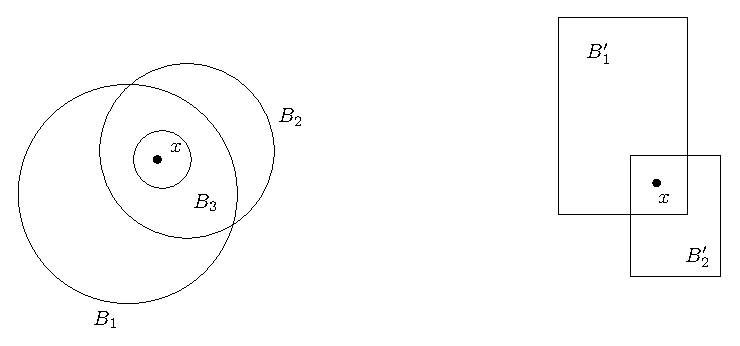
\includegraphics[width=\textwidth]{fig134.eps}
	\caption{Consider basis $\B$ of circular regions and basis $\B'$ of rectangular regions on $\R^2$. Intersection of two basis elements is another basis element for $\B'$, but not for $\B$.}
	\label{Fig:ExampleCircularBasis}
\end{figure}

\begin{exmp} We consider two different basis $\B$ and $\B'$ on set $X = \R^2$.
\begin{enumerate} 
	\item Consider basis $\B$ of circular regions for a topology on $\R^2$.
	\begin{align*}
		\B &= \{B(x_0,y_0,r) \subseteq \R^2: (x_0,y_0,r) \in \R^2 \times \R_+ \}, \text { where }\\
		B(x_0, y_0, r) &= \{ (x,y) \in \R^2: (x-x_0)^2 + (y-y_0)^2 < r^2\}.
	\end{align*}
	Generated topology $\T(\B)$ is given by
	\begin{align*}
		\T(\B) &= \{U \subseteq \R^2: \forall x \in U, \exists (x,y,r) \text{ such that } x \in B(x, y, r) \subseteq U \}.
	\end{align*}	
	\item Consider basis $\B'$ of rectangular regions for a topology on $\R^2$.
	\begin{align*}
		\B' &= \{B'(x_0,y_0,r) \subseteq \R^2: (x_0,y_0,r) \in \R^2 \times \R_+ \}, \text { where }\\
		B'(x_0, y_0, r) &= \{ (x,y) \in \R^2: \max\{\abs{x-x_0}, \abs{y-y_0}\} < r\}.
	\end{align*}
	Generated topology $\T(\B')$ is given by
	\begin{align*}
		\T(\B') &= \{U \subseteq \R^2: \forall x \in U, \exists (x,y,r) \text{ such that } x \in B'(x, y, r) \subseteq U \}.
	\end{align*}		
\end{enumerate}
 We show typical basis elements of $\B$ and $\B'$ in Figure~\ref{Fig:ExampleCircularBasis}. Observe that intersection of two basis elements $B_1, B_2 \in \B$ is not a basis element. But, by definition of basis, there exists an element $B_3 \subset B_1 \cap B_2$. 
%To see this, let $B_i = B(x_i,y_i,r_i), i \in [2]$ and $(x,y) \in B_1 \cap B_2$. Then, choosing 
	%\begin{align*}
	%r_3 = (r_1- \abs{x_1-x} \wedge \abs{y_1-y}) \wedge (r_2- \abs{x_2-x} \wedge \abs{y_2-y}), 
	%\end{align*}
	%we can show 
	%%\begin{align*}
	%$B_3 = B(x,y,r_3) \subseteq B_1 \cap B_2$.
	%%\end{align*}
On the other hand, intersection of two basis elements $B'_1, B'_2 \in \B'$ is a basis element itself. It can be shown that $\T(\B) = \T(\B')$.
%In particular, if $B'_i = B'(x_i,y_i,r_i), i \in [2]$. Then 
	%\begin{align*}
	%B'_1 \cap B'_2 = \{(x,y) \in \R^2: \}. 
	%\end{align*}
	%%consider the collection of all circular regions (interiors of circles) $\B$. 
\end{exmp}

\begin{exmp}
 Let $X$ be any set, then collection of all singletons is basis for \textbf{discrete topology} on $X$.
We will show collection of all singletons $\B = \{ \{x\}: x \in X\}$ is a basis.
	\begin{description}
		\item[Covering whole set.] Clearly $X = \cup_{x \in X} = \{x\}$.
		\item[Basis inside intersection.] Let $x \neq y$, then $\{x\} \cap \{y\} = \emptyset$, so second condition is vacuously true.
	\end{description}
\end{exmp}
\begin{lem}
Let $X$ be a set, and $\B$ be a basis for topology $\T$ on $X$. Then $\T$ equals the collection of all unions of elements of $\B$.
\end{lem}
\begin{proof} Let $\B = \{B_i: i \in I\}$. Since $\B \subseteq \T$ and $\T$ is a topology, hence for all $J \subseteq I$, we have $\cup_{j \in J}B_j \in \T$. That is, the collection of union of elements in $\B$ is in $\T$. 
Conversely, let $U \in \T$ be any open subset of $X$. For any $x \in X$, we can find $B_x \in \B$ such that $x \in B_x \subseteq U$ by definition of $\B$. Hence, we have $U = \cup_{x \in U}B_x$. That is, any element of $\T$ is union of basis elements in $\B$.
\end{proof}

\begin{rem} There is no unique way of representing an open set as union of basis elements. Thus, topological basis is quite different to linear algebra basis. 
\end{rem}
\end{document}  